\documentclass{article}
\usepackage[margin=1in, top = .8in, left=.8in]{geometry}
\usepackage{comment,hyperref}
\usepackage{amsmath, amssymb}
\usepackage{framed}
\usepackage{enumitem}
\usepackage{comment}
\usepackage{tikz,pgfplots}
\pgfplotsset{compat=1.15}

\usepackage{url}
\everymath{\displaystyle}
\newcommand{\R}{\mathbb{R}}
\newcommand{\N}{\mathbb{N}}
\everymath{\displaystyle}

\begin{document}
\begin{center}
\textbf{
    Sample problems with solutions for Homework 6}
\end{center}
    \begin{enumerate}
               \item The following is a graph of a function $g(x)$, which is a probability density function. The function $g(x)$ is $0$ on $(-\infty,0]$ and $[3,\infty)$.
                        \begin{center}
        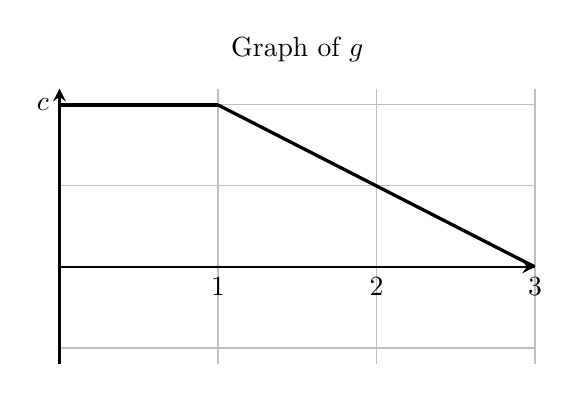
\begin{tikzpicture}
        \begin{axis}[
   	        xmin=0, xmax=3,
	        ymin=-1.2, ymax=2.2,
	        major tick length={0},
	        line width=1pt,
	        %xticks = {0,1,2,3,4},
 	        axis lines=center, height=2 in, width=3 in, grid=major,
 	        title = Graph of $g$,
 	        yticklabels = {, , ,,$c$}
	        ]
	    \addplot [black, smooth, very thick] plot coordinates {(0,2)(1,2)};
	    \addplot [black, smooth, very thick] plot coordinates {(1,2)(3,0)};

        \end{axis}
        \end{tikzpicture}
        \end{center}
                \begin{enumerate}
                    \item Find the value of $c$ needed to make $g$ a probability density function. thus determining the scale on the $y$-axis of the graph.
                    \item Write the formula for the cumulative distribution function as a piecewise function.
                    \item Graph the cumulative distribution function.
                    \item Find the probability that a number with this distribution lies between $2$ and $3$.
                \end{enumerate} \item For sample exercises on using L'H\^{o}pital's rule to find limits, see, for example
                \url{http://tutorial.math.lamar.edu/Classes/CalcI/LHospitalsRule.aspx}
                \item Determine if the integral $\int_1^\infty xe^{-x}\,dx$ converges or diverges.
                \item Determine if the integral $\int_2^\infty \frac{1}{\sqrt{x}-1}\,dx$ converges or diverges.
                \item Determine if $\int_1^\infty \frac{1}{xe^x}\,dx$ converges or diverges.
    \end{enumerate}
    \begin{center}
        \textbf{\Large{Solutions}}
    \end{center}
    \begin{enumerate}
    \item 
    \begin{enumerate}
    \item 
    For $g(x)$ to be a probability density function, we need the area under the curve of $g(x)$ to equal 1 on it's domain.  Using the graph, the area of under the curve is $c+\frac{1}{2}2c = 2c$, so $c$ must be $\frac{1}{2}$.
    \item Since $g(x)$ is a piece-wise function, we expect the same of its cumulative distribution function (CDF).   From $0$ to $1$, $g(x)=\frac{1}{2}$, so the CDF is
    \[\int_0^x \frac{1}{2}\ dt = \frac{1}{2}x\]
    Note that we changed the variable for $g$ to a $t$. From $1$ to $3$, we accumulate $\int_1^x \left(\frac{3}{4}-\frac{1}{4}t\right)\ dt$, and we need to add what we accumulated from 0 to 1. Therefore on this interval the cumulative distribution function, on the interval $[1,3]$ is given by
    \begin{eqnarray*}
    g(x) &=&\frac{1}{2} + \int_1^x \left(\frac{3}{4}-\frac{1}{4}t\right)\ dx \\[1em]
    &=& \frac{1}{2}+\left( \frac{3}{4}t-\frac{t^2}{8}\right)\biggr|_1^x \\[1em]
    &=& \frac{1}{2} +\left(\frac{3}{4}x-\frac{x^2}{8}\right)- \left(\frac{3}{4}-\frac{1}{8} \right) \\[1em]
    &=& -\frac{x^2}{8}+\frac{3}{4}x-\frac{1}{8} 
    \end{eqnarray*}
    \item Use this link to see the function:
    \item This probability is given by $g(3)-g(2)=\frac{1}{8}$
    \end{enumerate}
    \item[3.] This integration can be done with integration by parts, by which one can obtain the following:
    \[\lim_{t\to\infty} -xe^{-x}\biggr|_1^t + \int_1^t e^{-x}\ dx= \lim_{t\to\infty} -te^{-t} +1e^{-1} + \int_1^t e^{-x}\ dx\]
    The integral on the right we have already found to be $e^{-1}$, and the first limit can be shown to be zero using L'Hopital's or through an argument about growth rates. This means the value of the improper integral is $2e^{-1}$.  
    
    We should note that we can use the comparison test for this integral, because the comparison $x^{e^{-x}}>e^{-x}$ is not a useful one.
    \item[4.] This integral is not one we've seen the tools to integrate, and even if we did, we are only concerned with convergence or divergence. Let's compare the function we're integrating to  $\frac{1}{\sqrt{x}}$. Note that 
    \[\frac{1}{\sqrt{x}-1} > \frac{1}{\sqrt{x}}\]
    We showed in class, and you should verify that $\int_2^\infty \frac{1}{\sqrt{x}}\ dx$ diverges to infinity.  Since the function we are concerned with is strictly larger, we can use the comparison test for integrals to conclude that $\int_2^{\infty} \frac{1}{\sqrt{x}-1}dx$ also diverges to infinity.
    \item[5.] 
    \end{enumerate}
\end{document}